\section{Related Work}\label{related}
% %%%%%%%%%%%%%%%%%%%%
In this section, we first provide an overview of MPLS
(Sec.~\ref{related.overview}) before explaining how MPLS tunnels can be revealed
through active measurements (Sec.~\ref{related.revealing}).  We also position
this work regarding the state of the art.

\subsection{MPLS Overview}\label{related.overview}
%%%%%%%%%%%%%%%%%%%%%%%%%%%
The \dfn{Multiprotocol Label Switching} (MPLS)~\cite{rfc3031} was originally
designed to speed up the forwarding process. In practice, this was done with one
or more 32 bits \dfn{label stack entries} (LSE) inserted between the frame
header (Data-link layer) and the IP packet (Network layer).\footnote{MPLS is IP
layer protocol independent.} A given packet can manage several LSEs at the same
time. In this case, the packet is said having a \dfn{stack of labels}.  Each LSE
is made of four fields:  a 20-bit label value used for forwarding the packet to
the next router, a 3-bit Traffic Class field for quality of service (QoS),
priority, and Explicit Congestion Notification (ECN)~\cite{rfc5462}, a 1-bit
bottom of stack flag (when set the current label is the last in the
stack~\cite{rfc3032}), and an 8-bit time-to-live (LSE-TTL) field having the same
purpose as the IP-TTL field~\cite{rfc3443}.

MPLS routers, called \dfn{Label Switching Routers} (LSRs), exchange labelled
packets over \dfn{Label Switched Paths} (LSPs).   The first MPLS router
(\dfn{Ingress Label Edge Router}, or Ingress LER, i.e., the tunnel entry point)
adds the label stack, while the last MPLS router (\dfn{Egress Label Edge
Router}, or Egress LER, i.e., the tunnel exit point) removes the label stack.
In some cases, for performance reasons, the LSE stack may be removed by the
penultimate MPLS router (\dfn{penultimate hop popping}, PHP).  The Egress LER
then performs a classic IP lookup and forwards the traffic, reducing so the load
on the Egress LER (specially if the Egress LER is shared among several LSPs).
This means that, when using PHP, the tunnel exit is one hop before the Egress
LER. % In its most basic operation, LSPs are constructed along best effort routes
%using the \dfn{Label Distribution Protocol} (LDP~\cite{rfc5036}). More specific
%LSPs may be constructed for Traffic Engineering purposes, using an extension of
%the RSVP protocol, \dfn{RSVP-TE}~\cite{rfc3209}. In these two cases, the label
%stack contains only one LSE. A more complex usage is for Virtual Private Networks
%(VPN~\cite{rfc2917}), where LSPs are constructed using either LDP or RSVP-TE,
%and an additional LSE at the bottom of the label stack is used to specify a Virtual
%Routing Table at the Egress. In this case, the bottom of the stack is constant
%along an LSP, while the top of the stack is modified at each hop, as in the
%previous cases.

\subsection{Revealing MPLS Tunnels}\label{related.revealing}
% %%%%%%%%%%%%%%%%%%%%%%%%%%%%%%%%%%
MPLS routers may send ICMP \ttlexceeded messages when the LSE-TTL expires. In
order to debug networks where MPLS is deployed, routers may also implement
RFC4950~\cite{rfc4950}, an extension to ICMP allowing a router to embed an MPLS
LSE in an ICMP \ttlexceeded message. In that case, the router simply quotes the
MPLS LSE (or the LSE stack) of the received packet in the ICMP \ttlexceeded
message. RFC4950 is particularly useful for operators as it allows them to
verify the correctness of their MPLS tunnels and TE policy.

If the Ingress LER copies the IP-TTL value to the LSE-TTL field rather than
setting the LSE-TTL to an arbitrary value such as 255, LSRs along the LSP will
reveal themselves when using traceroute via ICMP messages even if they do not
implement RFC4950. Operators can configure this action using the \tpropagate
option provided by the router manufacturer~\cite{rfc3443} (while, to the best of
our knowledge, the RFC4950 is just a matter of implementation and cannot be
deactivated on recent routers supporting it). 

Using those two features, Sommers et al.~\cite{SOM11} provide an extensive study
of MPLS tunnels as observed in CAIDA's topology data.  In this data, they find
tunnels in 7\% of ASes, and the fraction is constant over the years of data
considered.  In addition, Sommers et al. propose a statistical methodology to
infer MPLS tunnels in archived data where ICMP extensions are not recorded.
Vanaubel et al.~\cite{Vanaubel15} propose a classification of path diversity
according to MPLS deployment.  Their classification reveals the actual usage of
MPLS (e.g., load balancing, traffic engineering) according to the inferred label
distribution protocol.  Finally, it has also been demonstrated that MPLS tunnels
may have an impact on Internet topology discovery tools.  For instance, the
presence of MPLS tunnels may interfere with load balancing
detection~\cite{BRICE07} or violate the destination-based
forwarding~\cite{Flach2012}.

Donnet et al.~\cite{Donnet12} propose a taxonomy of MPLS tunnels based on how
they react to \traceroute probes according to their compliance (or not) to
RFC4950 for MPLS and the \tpropagate option.  The classes proposed are:
\dfn{explicit tunnels} (i.e., \tpropagate and RFC4950 are enabled),
\dfn{implicit tunnels} (i.e., the router that pushes the MPLS label enables the
\tpropagate option but LSRs do not implement RFC4950), \dfn{opaque tunnels}
(i.e., the LH implements RFC4950 but the ingress LER does not enable the
\tpropagate option), and, finally, \dfn{invisible tunnels} (i.e., the ingress
LER does not enable the \tpropagate option and RFC4950 is not implemented by the
LH router).  Implicit and opaque tunnels can be revelead as follows:
\begin{enumerate}
  \item a quoted IP-TTL (\dfn{qTTL}) in ICMP \ttlexceeded messages $>1$ will
  likely reveal the \tpropagate option at the ingress LER of an LSP. For each
  subsequent \traceroute probe within an LSP, the qTTL will be one greater
  resulting in an increasing sequence of qTTL values in \traceroute.  This is
  illustrated in Fig.~\ref{validation.qTTLFig};
  \item  \#hops differences with the IP-TTL in \echoreply messages
  (\dfn{u-turn}).  It relies on the fact that LSRs along an LSP present an
  \textit{original label stack} default routing behavior: when the LSE-TTL
  expires, an LSR first sends the \ttlexceeded reply to the Egress LER which
  then forwards the reply on its own to the probing source, while an LSR
  replies to other probes using its own IP routing table if available. Summarizing, 
  $\textit{u-turn}=\text{TTL}_{\text{echo-reply}}-\text{TTL}_{\text{time-exceeded}}$.
  The expected u-turn value is in the form $[2L, 2L-2, 2L-4,..., 2]$ where $L$
  is the tunnel length and the array position corresponds to the LSR position
  within the LSP.
  \item opaque tunnels are revealed through an \textit{abnormal} LSE-TTL
  ($1<$LSE-TTL$<255$) returned by the LH in the \ttlexceeded reply.
\end{enumerate}

Additional study by Vanaubel et al.~\cite{VAN2013} shows that the probing
heuristic to detect implicit tunnels seems quite reliable.  However, u-turn
signatures are by definition more subject to false positives than qTTL ones. 
This is exactly what we tackle in this paper (and, consequently, our work is
complementary to Vanaubel et al.~\cite{VAN2013}): we want to test u-turn
signature accuracy.

%Figura u-turn
% \begin{figure*}[!t]
%   \begin{center}
%     \subfloat[Tunnel Length Distribution]{\label{hist_length}
%       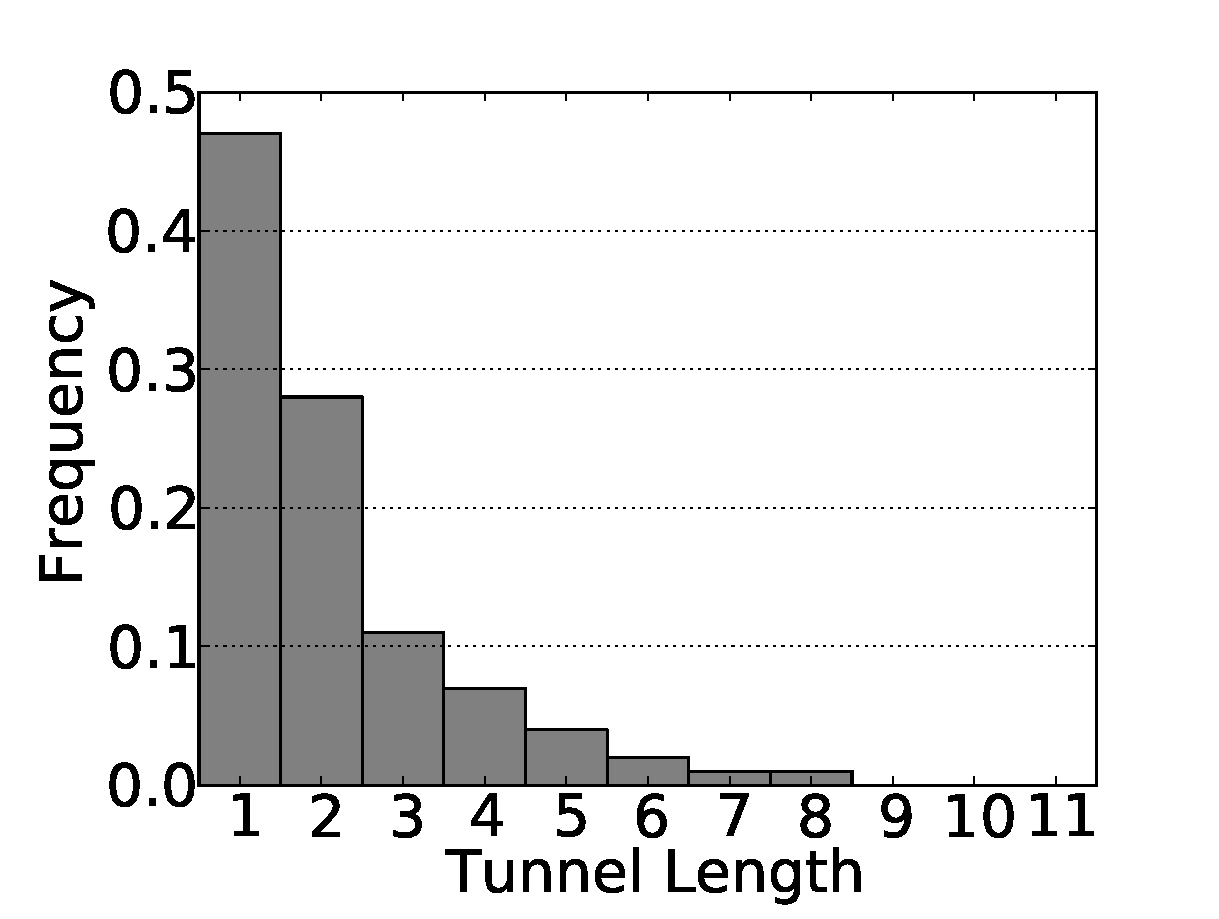
\includegraphics[width=6cm]{hist_length}}
%       \hfil
%     \subfloat[\textit{qTTL} and $n$-position comparison]{\label{n_vs_qttl}
%       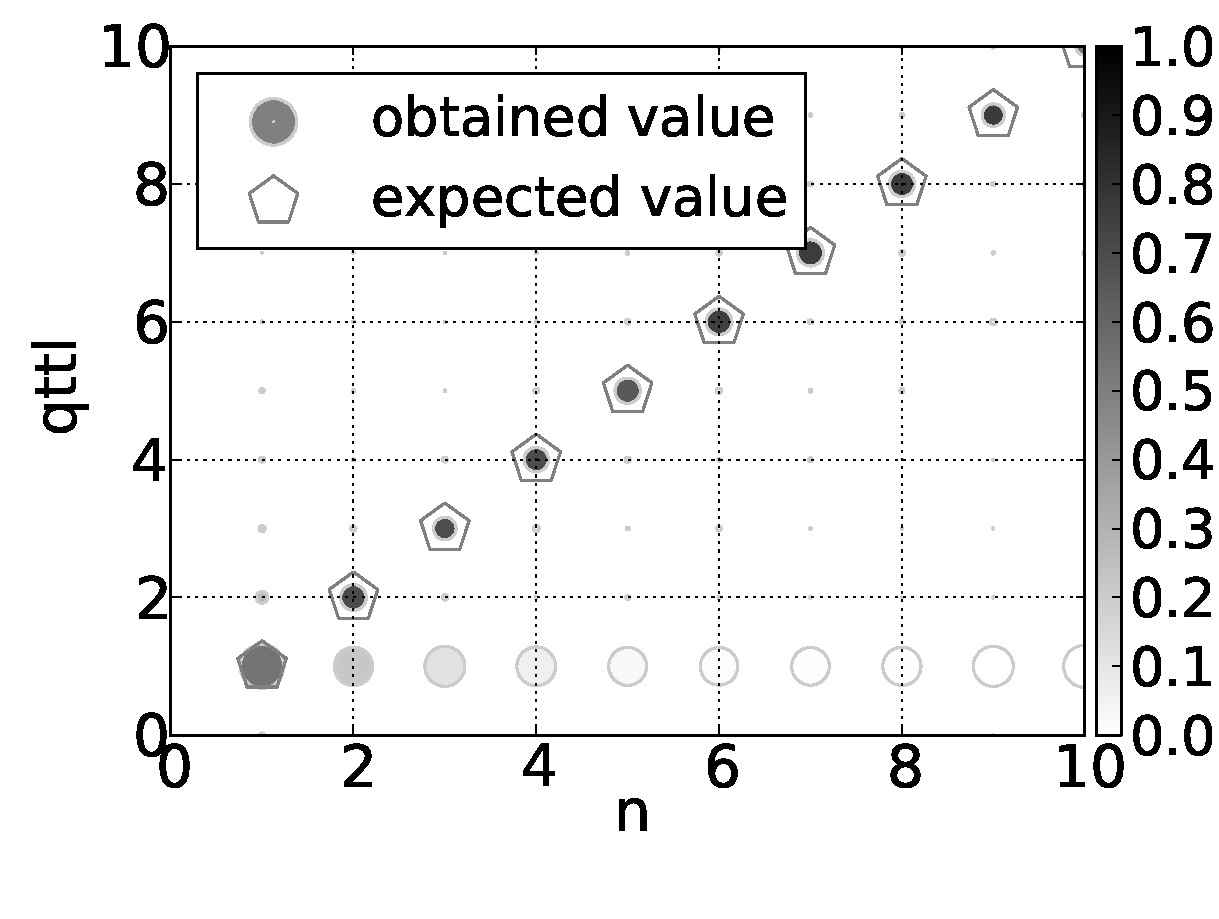
\includegraphics[width=6cm]{n_vs_qttl}} 
%       \hfil
%     \subfloat[\textit{u-turn} on LSRs revealed through RFC4950 and \textit{qTTL}]{\label{fig_uturn_a}
%       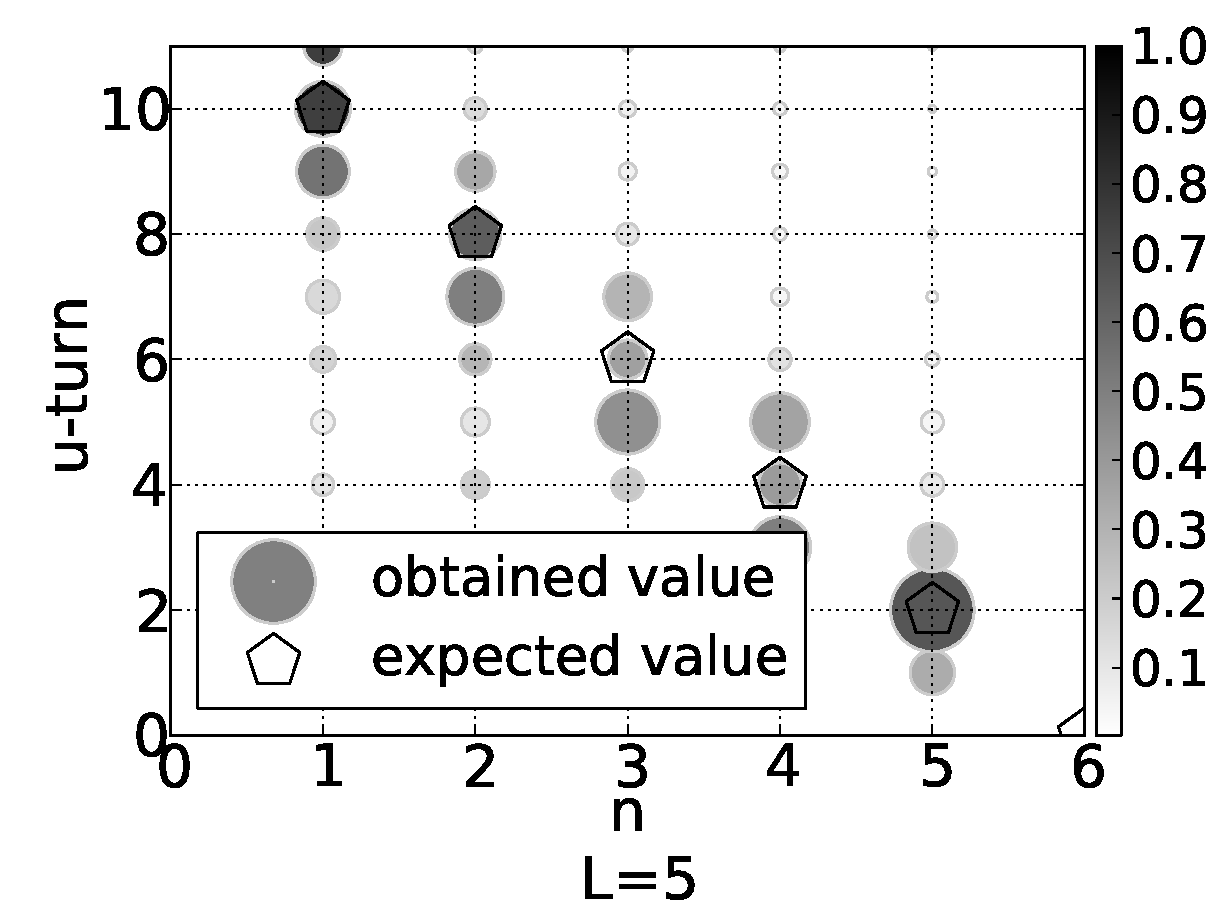
\includegraphics[width=6cm]{n_vs_uturn_L5_exp}}
%       \hfil
%     \subfloat[\textit{u-turn} on LSRs where no other signature was found]{\label{fig_uturn_b}
%       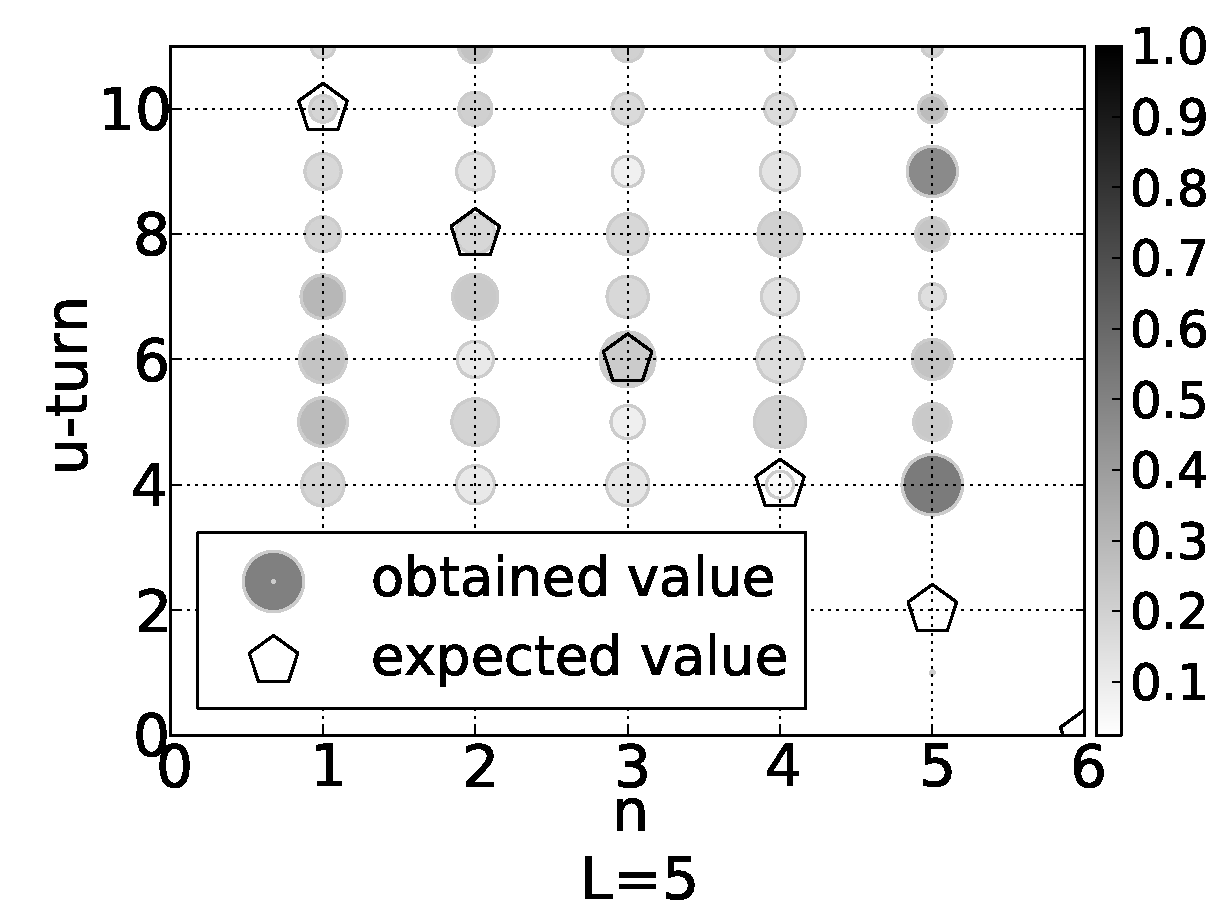
\includegraphics[width=6cm]{n_vs_uturn_L5}}
%    \end{center}
%   \caption{ Comparison between obtained and expected values for \textit{qTTL} and
%   \textit{u-turn} signatures. On figures (b), (c) and (d) the circle size in the scatter plot is related with the occurrence frequency of \textit{y-axis} values regarding each $n$-position. The
%   transparency of the circle is related with occurrence frequency of $n$-position  regarding each \textit{y-axis} value, e.g., on figure (b) for values where $n>1$, the biggest circles are mainly located on  $\textit{qTTL}=1$ and $\textit{qTTL}=n$ so this suggest that for a given $n$-position the \textit{qTTL} value usually takes either the value of $1$ or $n$; in the same way, the transparency value suggests that for a given \textit{qTTL} value the $n$-position usually takes the same \textit{qTTL} value.  \textbf{Figure (c)} and \textbf{Figure (d)} suggest that \textit{u-turn} value is overestimated. }
%   \label{ig_signatures}
% \end{figure*}

% \section{Related Work}\label{related}
% %%%%%%%%%%%%%%%%%%%%
% In the last years, MPLS~\cite{rfc3031} has been more and more investigated by
% the researchers.  This works mainly focused on MPLS tunnels detection. For
% instance, \Sommers et al.~\cite{SOM11} studied the MPLS deployment that is
% explicitly revealed through \textit{RFC 4950} extension. They also
% proposed a methodology to infer MPLS tunnels in archived data where ICMP extensions are not
% recorded. Most recently Donnet et al.~\cite{Donnet12} provided a
% taxonomy for MPLS tunnels and propose algorithms for detecting MPLS tunnels
% depending on the way that the LSRs react to the \textit{ttl-propagate} and
% \textit{RFC 4950} options. \ed{BD: I would remove this paragraph as it
% introduces concepts (RFC4950, LSRs, \ldots) that have not been }
% 
% It has also been studied the path diversity related with MPLS deployments. In
% this way, \textit{Vanaubel et al.} \cite{Vanaubel15} recently proposed and
% algorithm to better understand the path diversity and their usage within a given
% AS.
% 
% In this way, our work is complementary to tunnel detection issues. We test
% carefully some of the ways that reveals  MPLS tunnels and provided an analysis
% of how the MPLS tunnels impact the Internet Topology structure.

% \subsection{MPLS overview}\label{related.mpls}
% % %%%%%%%%%%%%%%%%%%%%%%%%% 
% MPLS \cite{RFC3031} was originally designed
% to speed up the forwarding process. In practice, this was done with one or more
% 32 bits Label Stack Entries (LSE) inserted between the frame header  and the IP
% packet.
% 
% In a MPLS network, packets are forwarded using an exact match lookup of a 20-bit
% label found in the LSE. An MPLS LSE also has a Time-To-Live (TTL) called LSE-TTL
% field and a Type-of-Service (ToS) field \cite{rfc1771}. At each MPLS hop, the
% label of the incoming packet is replaced by a corresponding outgoing label found
% in an MPLS switching table. A portion of a path where the forwarding decision is
% not anymore based on longest prefix matching but rather on MPLS features is
% known as an MPLS tunnel. A router with label switching capabilities is called
% Label Switching Router (LSR). A series of LSRs connected together form a Label
% Switched Path (LSP). The first router where the incoming packet includes a LSE
% is called ingress Label Edge Router (LER) and the last router that \textit{pops}
% the LSE is called Last Hop (LH).

% \subsection{Revealing MPLS tunnels} \label{related.signatures}
% 
% \textit{Donnet et al.} \cite{Donnet12} provided a taxonomy for MPLS tunnels
% revealed by traceroute and developed algorithms in order to detect it based on
% the way that LSR react to \textit{ttl-propagate}  and \textit{RFC 4950} option.
% Basically, their proposes two kind of visible MPLS tunnels: explicit tunnels and
% implicit tunnels.
% 
% Explicit tunnels are based on \textit{RFC 4950} implementation. MPLS routers may
% send ICMP time-exceeded messages when the LSE-TTL expires. The \textit{RFC 4950}
% is an extension to ICMP allowing a router to embed an MPLS LSE in an ICMP
% time-exceeded message. In that case, when the LSE-TTL expires on a MPLS router,
% it simply quotes the MPLS label stack in the ICMP \textit{time-exceeded}
% message.
% 
% Implicit tunnels discovery are based on two signatures detection: \textit{qttl}
% and \textit{u-turn} signature. The \textit{qttl} signature is relate with
% \textit{ttl-propagate} option. If  \textit{ttl-propagate} is implemented the LER
% copies the IP-TTL value to the LSE-TTL field rather than setting the LSE-TTL to
% an arbitrary value such as 255. In this way, the LSRs along the LSP will reveal
% themselves via ICMP messages even if they do not implement \textit{RFC 4950},
% i.e., if $\textit{qttl}>1$  the ICMP message was generated by an interfaces that
% belongs to an MPLS tunnel. The \textit{u-turn} signature relies on the fact that
% most LSRs in an LSP present a common behaviour: when the LSE-TTL expires, the
% LSR sends the ICMP \textit{time-exceeded} message to the LH router which then
% forwards the reply to the probing source, while an LSR replies to other probes
% such as  ICMP \textit{echo} packets using directly its own IP routing table if
% available. The variation between these two TTLs values is called \textit{u-turn}
% signature, i.e.,
% $\textit{u-turn}=TTL_{\text{echo-reply}}-TTL_{\text{time-exceeded}}$.  The
% expected \textit{u-turn} value in the form $[2L, 2L-2, 2L-4,..., 2]$ where $L$
% is the tunnel length and the array position correspond to the LSR position
% within the tunnel.
% 
% The \textit{qttl} signature ($\textit{qttl}>1$) is present just in MPLS
% behaviour.
% Commonly there is not another way to get a $\textit{qttl}>1$. However,
% \textit{u-turn} signature could be caused for another Internet issues such as
% police routing or load balancing paths, that produces different lengths in the
% return path.

% In this paper we consider that \textit{RFC 4950} implementation and
% \textit{qttl} signature are highly reliable methods to reveal MPLS tunnels and
% we mainly focus on to test \textit{u-turn} signature accuracy.

% \subsection{Diversity on MPLS paths}
% 
% \textit{Vanaubel et al.} \cite{SOM11} proposed a classification of path
% diversity on MPLS deployments. Their algorithm allow to classify the kind of
% diversity path regarding the behaviour of mpls labels on explicit tunnels. The
% authors propose basically a path classification based on physical diversity
% i.e., paths with different IP interfaces; and logical diversity i.e., paths with
% the same IP interfaces but different labels. The work show a detailed study of
% path diversity over the top of ASs with most MPLS tunnels discovered.       
